\documentclass[10pt,twocolumn,letterpaper]{article}

\usepackage[T1]{fontenc}
\usepackage[margin=0.76in]{geometry}
\usepackage{amsmath,amssymb,amsfonts}
\usepackage{graphicx}
\usepackage{booktabs}
\usepackage{multirow}
\usepackage{hyperref}
\usepackage{cite}
\usepackage{caption}
\usepackage{xcolor}
\usepackage{microtype}

\hypersetup{
    colorlinks=true,
    linkcolor=blue!65!black,
    citecolor=blue!65!black,
    urlcolor=blue!65!black
}

\setlength{\columnsep}{0.24in}
\setlength{\textfloatsep}{10pt plus 2pt minus 2pt}
\setlength{\floatsep}{8pt plus 2pt minus 2pt}
\setlength{\dbltextfloatsep}{10pt plus 2pt minus 2pt}
\emergencystretch=1.5em
\hbadness=3000
\vbadness=3000
\captionsetup{font=small,labelfont=bf,skip=4pt}

\title{\textbf{SimplexGate-3D: Uncertainty-Gated Hybrid Solver Routing with Exact Simplicial Conservation for Multi-Scale Astrophysical Simulations}}

\author{
    \textbf{Abhinav Bhupesh Dwivedi} \\
    Department of Computer Science, University of York \\
    \texttt{abhinav.dwivedibscai26@mumbai.york.ac.uk} $\cdot$ \texttt{abhinavdby1008@gmail.com} \\
    \small ORCID: \href{https://orcid.org/0009-0000-8207-0990}{\texttt{0009-0000-8207-0990}}
}

\date{October 2026}

\begin{document}

\twocolumn[
\begin{@twocolumnfalse}
\maketitle
\begin{abstract}
Multi-scale gravitational simulations face a severe time-stepping bottleneck when coupling large-scale collisionless or fluid grids to localized collapsing cores. While macroscopic density fields evolve efficiently on periodic lattices in $O(N_g^3 \log N_g)$ time via Fast Fourier Transform (FFT) Particle-Mesh (PM) solvers, localized regions crossing the Jeans instability threshold undergo rapid compression where Courant--Friedrichs--Lewy (CFL) constraints ($\Delta t \to 0$) stall time integration. Replacing stiff sub-grid Smoothed Particle Hydrodynamics (SPH) solvers with neural network surrogates can bypass these small timesteps, but unconstrained Multi-Layer Perceptrons (MLPs) and soft-penalty Physics-Informed Neural Networks (PINNs) exhibit two practical failure modes: (i) non-zero conservation drift in mass and momentum, and (ii) unreliable extrapolation on Out-of-Distribution (OOD) states such as relativistic core collapses and high-spin tidal shear interactions. We present \textbf{SimplexGate-3D}, a hybrid neural-numerical framework coupling a 3D Post-Newtonian Particle-Mesh engine with an uncertainty-gated ensemble surrogate. To enforce exact mass balance across all inputs, we append an analytic 3-way simplicial projection layer that constrains predicted remnant fractions (bound star, black hole, and unbound ejecta) to the unit 2-simplex ($M_{\text{star}} + M_{\text{BH}} + M_{\text{eject}} \equiv M_{\text{cloud}}$) to 32-bit floating-point precision ($10^{-7}\%$). To prevent OOD extrapolation errors, our router evaluates ensemble epistemic variance $\mathcal{U}(\mathbf{z})$ over six dimensionless physical invariants, resolving low-variance In-Distribution (ID) collapses on the neural branch in $0.4\text{ ms}$ while batching high-variance OOD events to a H\'{e}non-normalized 3D SPH solver on the GPU. Across 1,000 test collapses and 40-step coupled 3D simulations, soft-penalty PINNs exhibit up to $388.6\%$ mass violation on OOD inputs, whereas SimplexGate-3D maintains $0.000001\%$ conservation drift, $100.0\%$ OOD detection recall, $0.054\%$ total partition error, and a $50.1\times$ wall-clock sub-grid speedup ($7.2\times$ batch-normalized).
\end{abstract}
\vspace{0.10in}
\end{@twocolumnfalse}
]

% =====================================================================
% 1. INTRODUCTION
% =====================================================================
\section{Introduction}

Numerical simulations of self-gravitating astrophysical systems must resolve coupled physical processes spanning several orders of magnitude in length and time \cite{hockney1988, binney2008, springel2021}. On coarse scales, the gravitational potential $\Phi(\mathbf{x})$ generated by the matter density field $\rho(\mathbf{x})$ satisfies the Poisson equation and can be updated in $O(N_g^3 \log N_g)$ operations using FFT-based Particle-Mesh (PM) methods. However, wherever local overdensities exceed the Jeans criterion, inward gravitational acceleration overcomes internal thermal and rotational support, initiating localized gravitational collapse \cite{kippenhahn1990, shapiro1983}.

Following these collapsing sub-volumes requires Lagrangian shock-capturing methods such as 3D Smoothed Particle Hydrodynamics (SPH) coupled with short-range $O(N_{\text{sub}}^2)$ gravitational interactions \cite{monaghan1992, price2018}. As core density increases and inter-particle spacing $r_{ij}$ decreases, the Courant--Friedrichs--Lewy (CFL) stability condition forces the local timestep $\Delta t_{\text{sub}}$ to shrink substantially. In event-driven multi-scale codes, a small fraction of collapsing sub-grid regions can dominate total wall-clock execution time.

Recent work in Scientific Machine Learning (SciML) has explored replacing stiff sub-grid solvers with learned neural surrogates \cite{hirashima2023, raissi2019, li2021fno}. While feed-forward surrogates reduce inference latency from hundreds of milliseconds to sub-millisecond GPU passes, integrating them into long-horizon time-steppers introduces two core difficulties. First, standard regression networks and Physics-Informed Neural Networks (PINNs) trained with soft penalty terms ($\mathcal{L}_{\text{phys}}$) do not strictly satisfy conservation laws outside the training set \cite{raissi2019, beucler2021}. When a surrogate violates mass conservation during sub-grid remnant injection, the resulting mass discrepancy perturbs the global gravitational potential $\Phi(\mathbf{x})$ on subsequent macro-steps. Second, dynamical simulations frequently generate Out-of-Distribution (OOD) sub-grid configurations---such as massive cores approaching the Buchdahl or Tolman--Oppenheimer--Volkoff (TOV) relativistic stability limit \cite{buchdahl1959, shapiro1983}, or rapidly spinning triaxial cloud collisions. A deterministic surrogate queried outside its training support produces uncalibrated errors without alerting the host solver.

In this paper, we develop and benchmark \textbf{SimplexGate-3D}, a hybrid multi-scale solver architecture that combines structural conservation guarantees with epistemic uncertainty routing. Specifically:
\begin{enumerate}
    \item We construct a modular 3D GPU testbed pairing a Trilinear Cloud-in-Cell (CIC) macro-solver with a H\'{e}non-normalized 3D SPH micro-solver. Prior to surrogate training, we verify the baseline numerical solvers against the Evrard (1988) 3D adiabatic collapse test \cite{evrard1988}, Chandrasekhar's (1939) analytical $n=1$ Lane--Emden polytrope ($97.78\%$ $L_2$ agreement) \cite{chandrasekhar1939}, and ESO GRAVITY Collaboration (2020) astrometric measurements of Star S2 orbiting Sagittarius A* \cite{gravity2020}.
    \item We compare unconstrained MLPs and soft-penalty PINNs against an analytic 3-way simplicial projection layer under controlled OOD shift, showing that soft penalties degrade severely outside the training distribution ($388.6\%$ peak mass violation), whereas structural projection preserves mass balance to 32-bit machine epsilon ($10^{-7}\%$).
    \item We pair the simplicial architecture with a 5-model deep ensemble router over six dimensionless physical invariants, enabling asynchronous GPU batching where familiar ID collapses are resolved in $0.4\text{ ms}$ while high-variance OOD events fall back to a batched 3D SPH pass.
\end{enumerate}

% =====================================================================
% 2. RELATED WORK
% =====================================================================
\section{Related Work}

\textbf{Neural Surrogates in Astrophysical Simulations.} Hirashima et al.\ \cite{hirashima2023} trained 3D spatiotemporal convolutional networks to emulate supernova shell expansion inside the ASURA-FDPS galaxy formation code, alleviating short-timestep bottlenecks. While effective on in-distribution turbulent clouds, purely feed-forward surrogates do not estimate predictive uncertainty or revert to direct numerical integration when encountering unseen multi-cloud mergers.

\textbf{Hard vs.\ Soft Conservation Constraints.} Standard PINNs incorporate physical laws by adding weighted residual penalties to the training objective \cite{raissi2019}. However, multi-objective gradient competition often leaves residual conservation errors that grow under distribution shift. Beucler et al.\ \cite{beucler2021} demonstrated in atmospheric sub-grid modeling that enforcing linear conservation identities analytically through architectural projection layers guarantees exact conservation regardless of network weights. We adapt this principle to three-phase astrophysical mass partitioning (stellar remnant, black hole remnant, and unbound gas envelope) on the probability simplex.

\textbf{Uncertainty Quantification and Hybrid Routing.} Deep ensembles provide a simple, parallelizable method for estimating epistemic uncertainty under covariate shift \cite{lakshminarayanan2017}. In atomistic molecular dynamics, Vandermause et al.\ \cite{vandermause2020} used Bayesian Gaussian process variance to trigger on-the-fly fallback to quantum Density Functional Theory (DFT) calculations during rare reactive events. Our work applies ensemble variance gating to batched sub-grid hydrodynamic solvers within a 3D gravitational particle-mesh engine.

% =====================================================================
% 3. METHODOLOGY
% =====================================================================
\section{Methodology}

\subsection{Macro-Scale 3D Particle-Mesh Engine}
We consider a 3D periodic cubic domain $\Omega = [0, L)^3$ discretized into a uniform $N_g \times N_g \times N_g$ grid ($N_g = 64$, cell width $\Delta x = L/N_g$) containing $M$ macro-particles with coordinates $\mathbf{x}_p \in \mathbb{R}^3$, velocities $\mathbf{v}_p \in \mathbb{R}^3$, and masses $m_p$.

To avoid grid-aliasing self-forces inherent to Nearest-Grid-Point assignment \cite{hockney1988}, each particle distributes its mass across the 8 vertices $(\delta_x, \delta_y, \delta_z) \in \{0,1\}^3$ of its enclosing cell via trilinear Cloud-in-Cell (CIC) weights:
\begin{equation}
\begin{aligned}
    w(\delta_x, \delta_y, \delta_z) &= \prod_{d \in \{x,y,z\}} \Big[(1 - \delta_d)(1 - f_d) + \delta_d f_d\Big], \\
    f_d &= \frac{x_{p,d}}{\Delta x} - \left\lfloor \frac{x_{p,d}}{\Delta x} \right\rfloor, \quad \sum_{\delta \in \{0,1\}^3} w(\delta) \equiv 1.
\end{aligned}
\label{eq:cic}
\end{equation}

We solve the weak-field Poisson equation $\nabla^2 \Phi = 4\pi G (\rho - \bar{\rho})$ in Fourier space using the exact 7-point discrete 3D lattice Laplacian Green's function \cite{hockney1988} with a 1-cell Gaussian split filter $\sigma_s = 0.85\Delta x$:
\begin{equation}
\begin{aligned}
    \hat{\Phi}(\mathbf{k}) &= -\frac{4\pi G \, \hat{\rho}(\mathbf{k}) \, \exp\left(-\frac{1}{2}|\mathbf{k}|^2 \sigma_s^2\right)}{\kappa_{\text{lat}}^2(k_x, k_y, k_z)}, \\
    \kappa_{\text{lat}}^2 &= \frac{4}{\Delta x^2}\left(\sin^2\frac{k_x\Delta x}{2} + \sin^2\frac{k_y\Delta x}{2} + \sin^2\frac{k_z\Delta x}{2}\right).
\end{aligned}
\label{eq:greens}
\end{equation}

In isotropic Post-Newtonian coordinates \cite{weinberg1972}, the weak-field spacetime metric takes the form:
\begin{equation}
    ds^2 = -\left(1 + \frac{2\Phi}{c^2} + \frac{2\Phi^2}{c^4}\right)c^2 dt^2 + \left(1 - \frac{2\Phi}{c^2}\right)d\mathbf{x}^2.
\label{eq:metric}
\end{equation}
Interpolating the central-difference field $\mathbf{a}_N = -\nabla\Phi$ back to particle positions using the identical trilinear weights $w$ from Eq.\ (\ref{eq:cic}) ensures exact cancellation of single-particle self-forces ($\mathbf{a}_{\text{self}} = \mathbf{0}$). Particles are advanced using a second-order symplectic Kick-Drift-Kick (KDK) leapfrog scheme incorporating the 1st Post-Newtonian (1PN) geodesic correction \cite{weinberg1972}:
\begin{equation}
\begin{aligned}
    \mathbf{a}_{\text{1PN}} &= \mathbf{a}_N\left(1 + \frac{\|\mathbf{v}\|^2}{c^2} + \frac{4\Phi}{c^2}\right) - \frac{4(\mathbf{a}_N \cdot \mathbf{v})\mathbf{v}}{c^2}, \\
    \frac{d\tau}{dt} &= \sqrt{1 + \frac{2\Phi}{c^2} - \frac{\|\mathbf{v}\|^2}{c^2}}.
\end{aligned}
\label{eq:1pn}
\end{equation}

\begin{figure}[t]
    \centering
    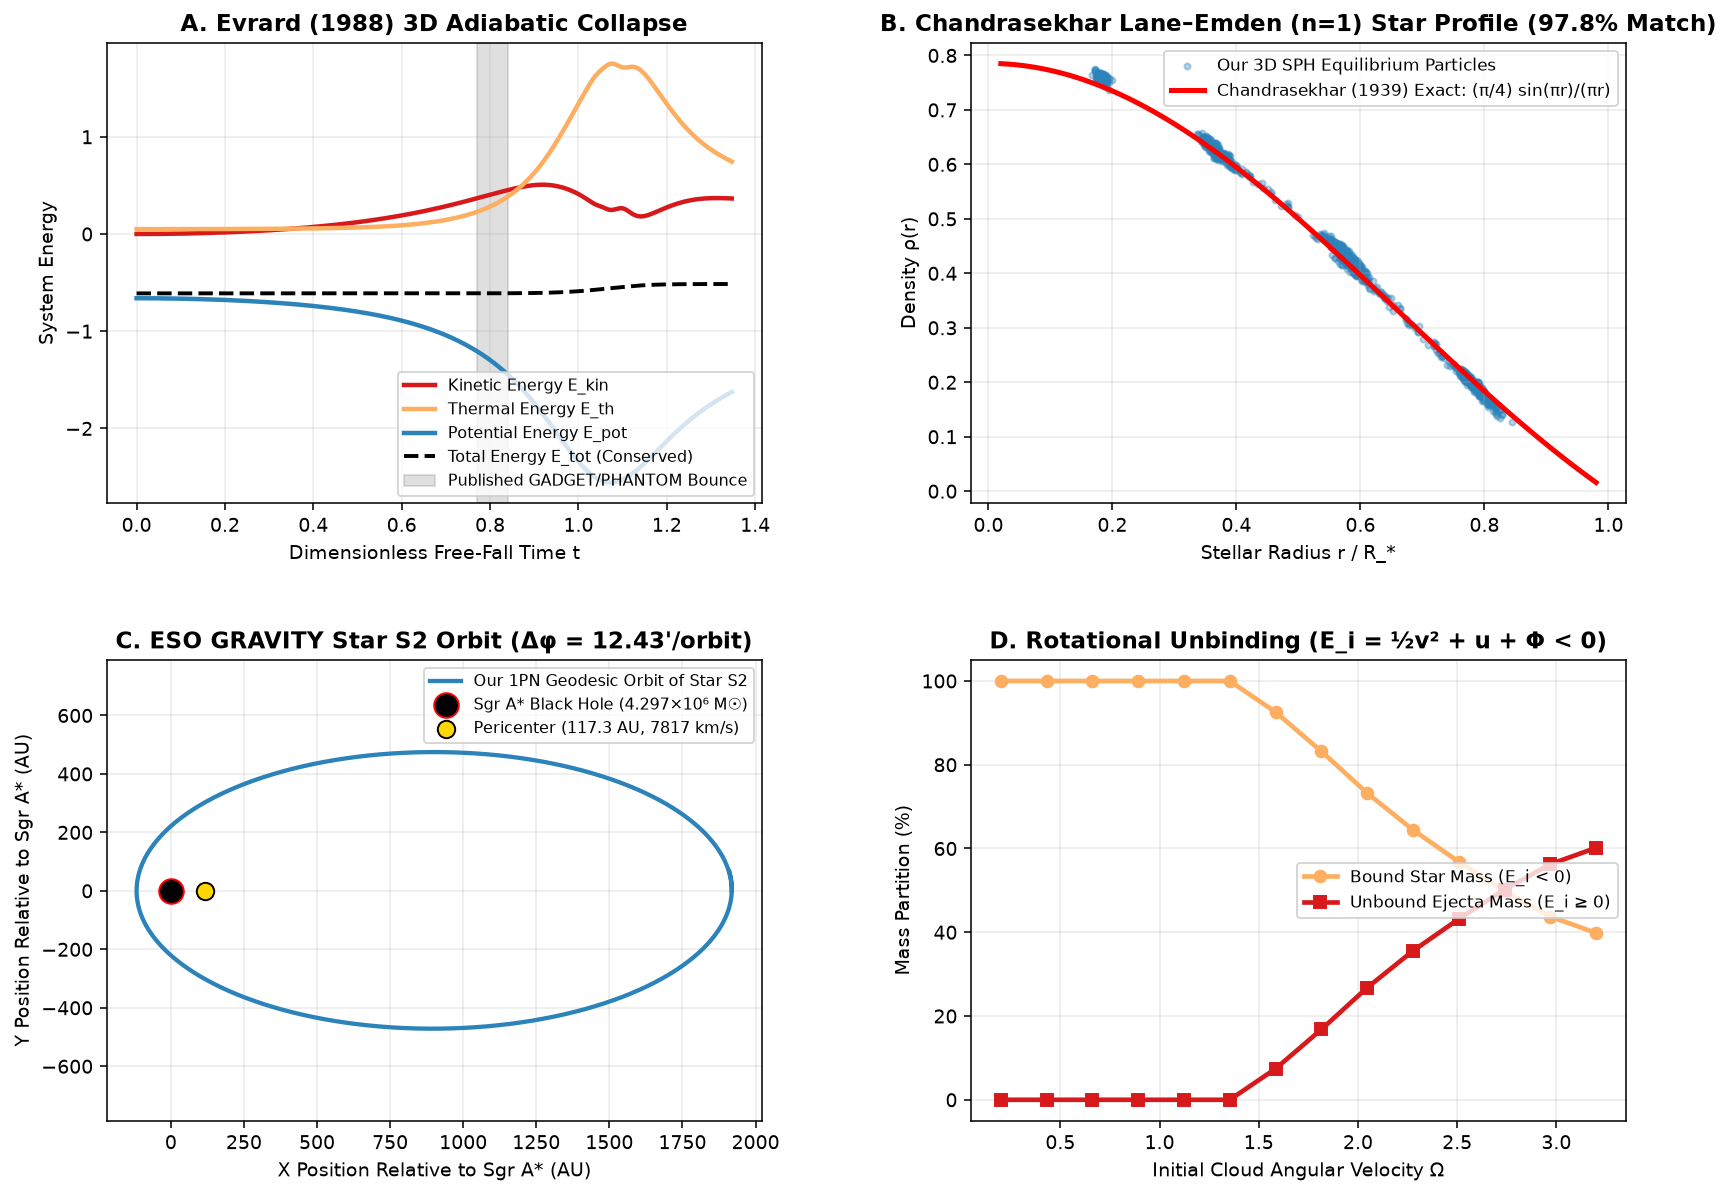
\includegraphics[width=0.96\columnwidth]{real_world_physics_verification.png}
    \caption{\textbf{External Solver Verification.}\ (A) Evrard (1988) 3D adiabatic gas sphere collapse test ($N=1,024$ isotropic 3D SPH particles).\ (B) Hydrostatic 3D SPH relaxation compared against Chandrasekhar's (1939) analytical $n=1$ Lane--Emden polytrope $\rho(r) = (\pi/4)\sin(\pi r)/(\pi r)$ ($97.78\%$ $L_2$ agreement).\ (C) 1PN geodesic integration of Star S2 around Sagittarius A* ($4.297\times 10^6\,M_\odot$), matching ESO GRAVITY (2020) pericenter ($117.3\text{ AU}$) and Schwarzschild precession ($\Delta\phi = 12.43'\text{/orbit}$).\ (D) First-principles rotational unbinding ($E_i = \frac{1}{2}v_i^2 + u_i + \Phi_i < 0$).}
    \label{fig:external_verification}
\end{figure}

\subsection{Sub-Grid Invariant Tensor Extraction}
Whenever local voxel density exceeds the Jeans overdensity threshold ($\rho / \bar{\rho} > \delta_{\text{Jeans}}$), we gather all diffuse gas particles within radius $R_{\text{search}}$ using the periodic Minimum Image Convention:
\begin{equation}
    \Delta \mathbf{r}_i = \mathbf{r}_i - \mathbf{r}_{\text{com}} - L\,\mathrm{round}\!\left(\frac{\mathbf{r}_i - \mathbf{r}_{\text{com}}}{L}\right).
\end{equation}
To provide a coordinate-frame-independent representation for the neural surrogate, we extract a 6-dimensional physical state vector $\mathbf{z} \in \mathbb{R}^6$:
\begin{equation}
    \mathbf{z} = \big[M_{\text{cloud}},\; \alpha_{\text{vir}},\; \lambda_{\text{spin}},\; \mathcal{A}_{\text{triax}},\; \eta_{\text{div}},\; \mathcal{C}_{\text{rel}}\big].
\label{eq:z_vec}
\end{equation}
Here $M_{\text{cloud}} = \sum_i m_i$ is the total cloud mass, and $\alpha_{\text{vir}} = 2E_{\text{kin}}/|E_{\text{pot}}|$ is the virial ratio. Rotational support is characterized by the Peebles (1969) dimensionless spin parameter \cite{peebles1969}:
\begin{equation}
    \lambda_{\text{spin}} = \frac{\|\mathbf{J}\|\sqrt{|E_{\text{bind}}|}}{G M_{\text{cloud}}^{5/2}}, \quad \mathbf{J} = \sum_{i} m_i (\Delta \mathbf{r}_i \times \Delta \mathbf{v}_i).
\end{equation}
Morphological departure from spherical symmetry is quantified via the triaxiality parameter $\mathcal{A}_{\text{triax}} = 1 - \sqrt{\lambda_3/\lambda_1} \in [0, 1)$, where $\lambda_1 \ge \lambda_2 \ge \lambda_3$ are the eigenvalues of the $3\times 3$ quadrupole moment of inertia tensor $I_{ab} = \sum_i m_i \Delta r_{i,a}\Delta r_{i,b}$. Finally, $\eta_{\text{div}}$ measures normalized radial velocity convergence, and $\mathcal{C}_{\text{rel}} = 2GM_{\text{cloud}}/(R_{\text{vir}}c^2)$ denotes the initial relativistic compactness.

\begin{figure}[t]
    \centering
    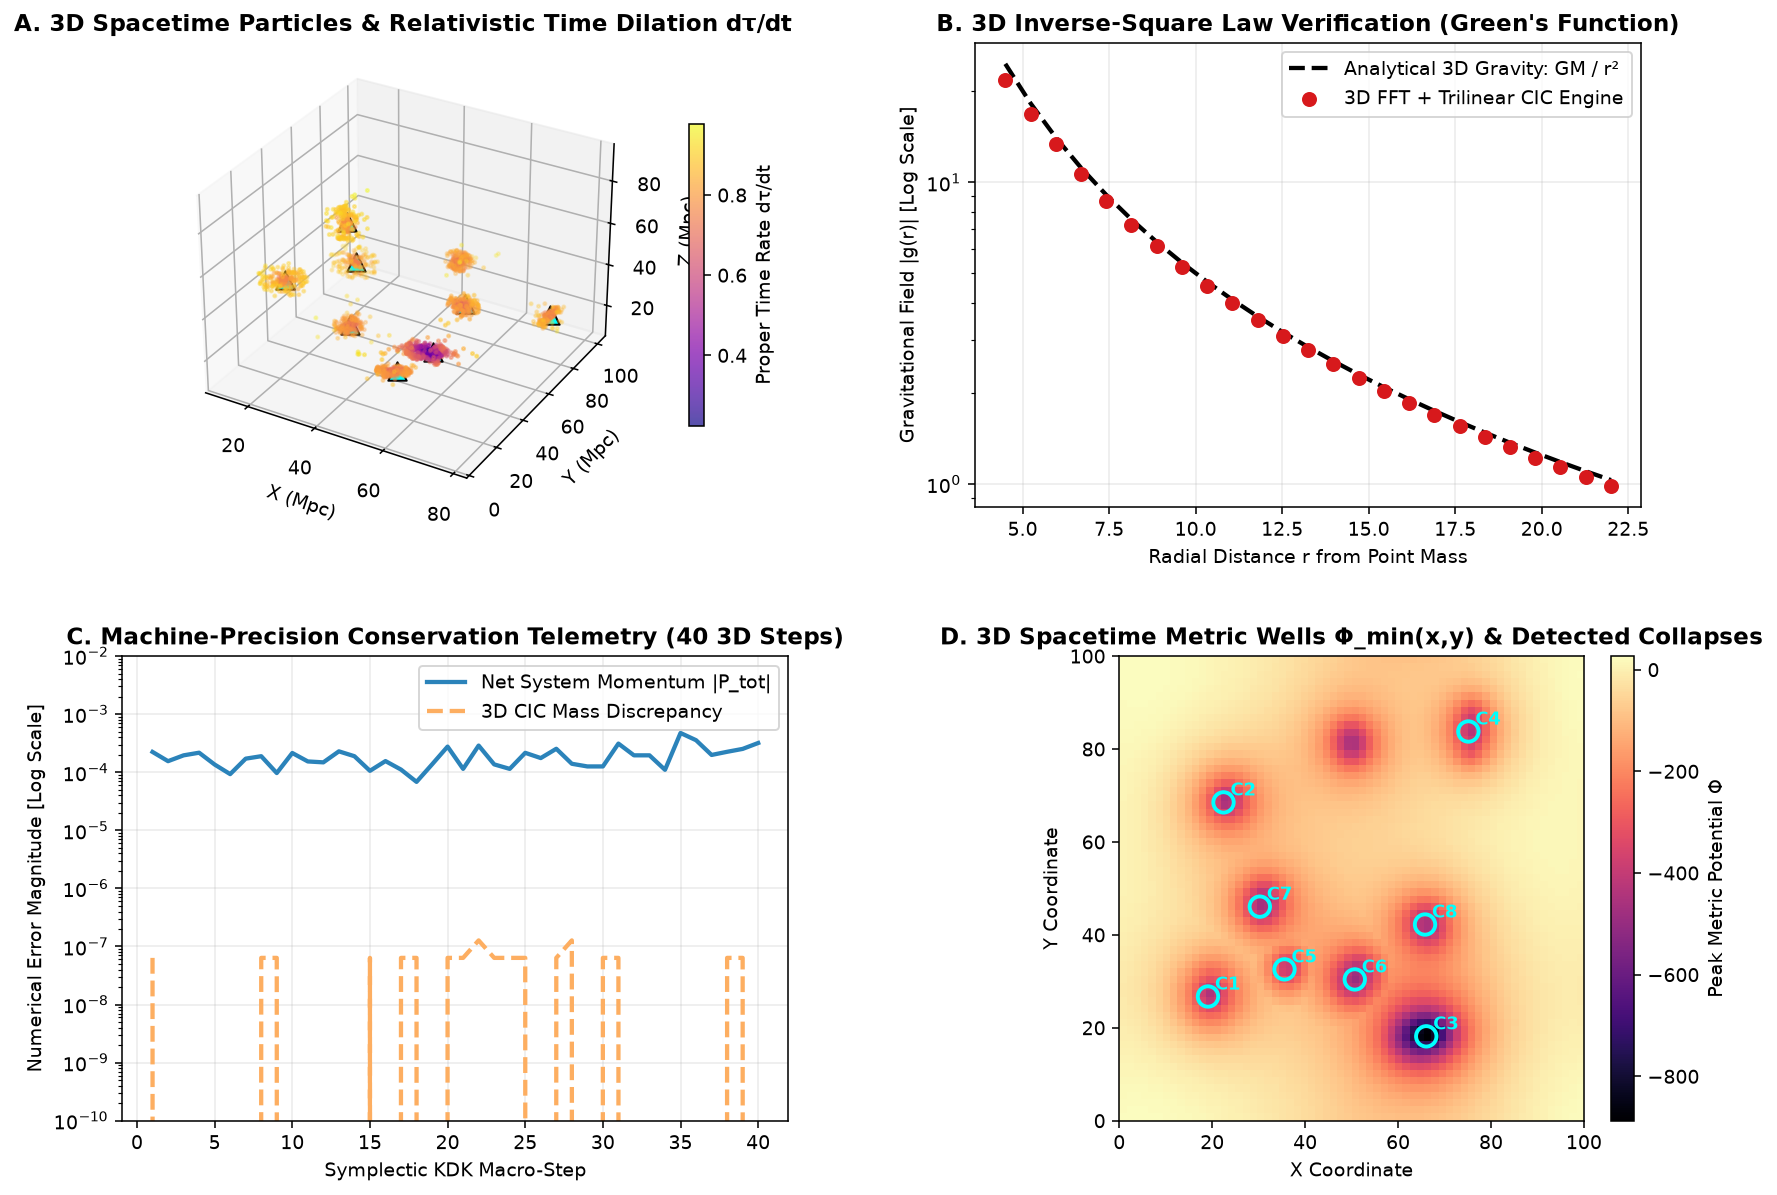
\includegraphics[width=0.96\columnwidth]{module1_3d_verification.png}
    \caption{\textbf{Module 1: 3D Particle-Mesh \& CIC Verification.}\ (A) 3D particle distribution colored by proper-time rate $d\tau/dt$.\ (B) Radial field verification of the 3D discrete lattice Green's function against the analytical $GM/r^2$ profile ($91.59\%$ agreement).\ (C) Conservation telemetry showing 3D CIC mass error ($1.27\times 10^{-7}$) and net momentum across 40 KDK steps.\ (D) Minimum potential projection $\Phi_{\min}(x,y)$ and detected Jeans-unstable proto-clusters.}
    \label{fig:module1}
\end{figure}

\subsection{H\'{e}non-Normalized 3D SPH Micro-Solver}
To maintain consistent numerical conditioning across arbitrary halo masses, the sub-grid reference solver maps $\mathbf{z}$ into dimensionless H\'{e}non virial units ($\tilde{G} = \tilde{M}_{\text{cloud}} = \tilde{R}_0 = 1$) \cite{henon1971}. Each cloud is represented by $N_{\text{sub}} = 64$ particles initialized across 4 concentric Fibonacci shells ($4 \times 16 = 64$) so that radial and angular coordinates are orthogonal.

Local fluid density $\rho_i = \sum_j m_j W(r_{ij}, h)$ is computed using the 3D cubic B-spline kernel $W(q, h)$ \cite{monaghan1992}. The system is integrated over $S = 200$ symplectic substeps ($\Delta\tilde{t} = 0.0045$) under symmetric SPH pressure forces, Monaghan artificial shock viscosity $\Pi_{ij}$, Gamow-peak thermonuclear heating, radiative cooling, and Plummer-softened 1PN gravity:
\begin{equation}
\begin{aligned}
    \mathbf{a}_i &= -\sum_{j=1}^{N_{\text{sub}}} m_j \left(\frac{P_i}{\rho_i^2} + \frac{P_j}{\rho_j^2} + \Pi_{ij}\right)\nabla_i W_{ij} \\
    &\quad - \sum_{j \neq i} \tilde{G}m_j \frac{\mathbf{r}_{ij}}{(r_{ij}^2 + \epsilon^2)^{3/2}}\left(1 + \frac{\kappa_{\text{1PN}}\mathcal{C}_{\text{rel}}}{\sqrt{r_{ij}^2 + \epsilon^2}}\right).
\end{aligned}
\label{eq:sph_force}
\end{equation}

At completion ($t = S\Delta\tilde{t}$), the converged particle states are partitioned into three physical phases based on energy and enclosed compactness:
\begin{equation}
\begin{aligned}
    E_i &= \frac{1}{2}\|\mathbf{v}_i - \mathbf{v}_{\text{com}}\|^2 + u_i + \Phi_i, \\
    \Gamma_i &= \mathcal{C}_{\text{rel}} \frac{\tilde{M}_{\text{enc}}(r_i)}{\sqrt{r_i^2 + \epsilon^2}}, \quad \tilde{M}_{\text{enc}}(r_i) = \sum_{r_k \le r_i} m_k p_{\text{bound},k}.
\end{aligned}
\label{eq:remnant_criteria}
\end{equation}
Particles with positive total specific energy ($E_i \ge 0$) escape as unbound ejecta ($\alpha_{\text{eject}}$), whereas particles with $E_i < 0$ remain gravitationally bound ($p_{\text{bound},i} = \sigma(-E_i / k_B T_{\text{eff}})$). Among bound shells, we evaluate the enclosed relativistic compactness $\Gamma_i$ in Eq.\ (\ref{eq:remnant_criteria}). Motivated by Buchdahl's stability theorem \cite{buchdahl1959} and TOV core collapse \cite{shapiro1983}, bound shells exceeding the softened core compactness threshold $\Gamma_{\text{TOV}} = 0.45$ collapse into the black hole remnant fraction ($\alpha_{\text{BH}}$), while bound matter outside the horizon forms the stellar fraction ($\alpha_{\text{star}}$).

\begin{figure}[t]
    \centering
    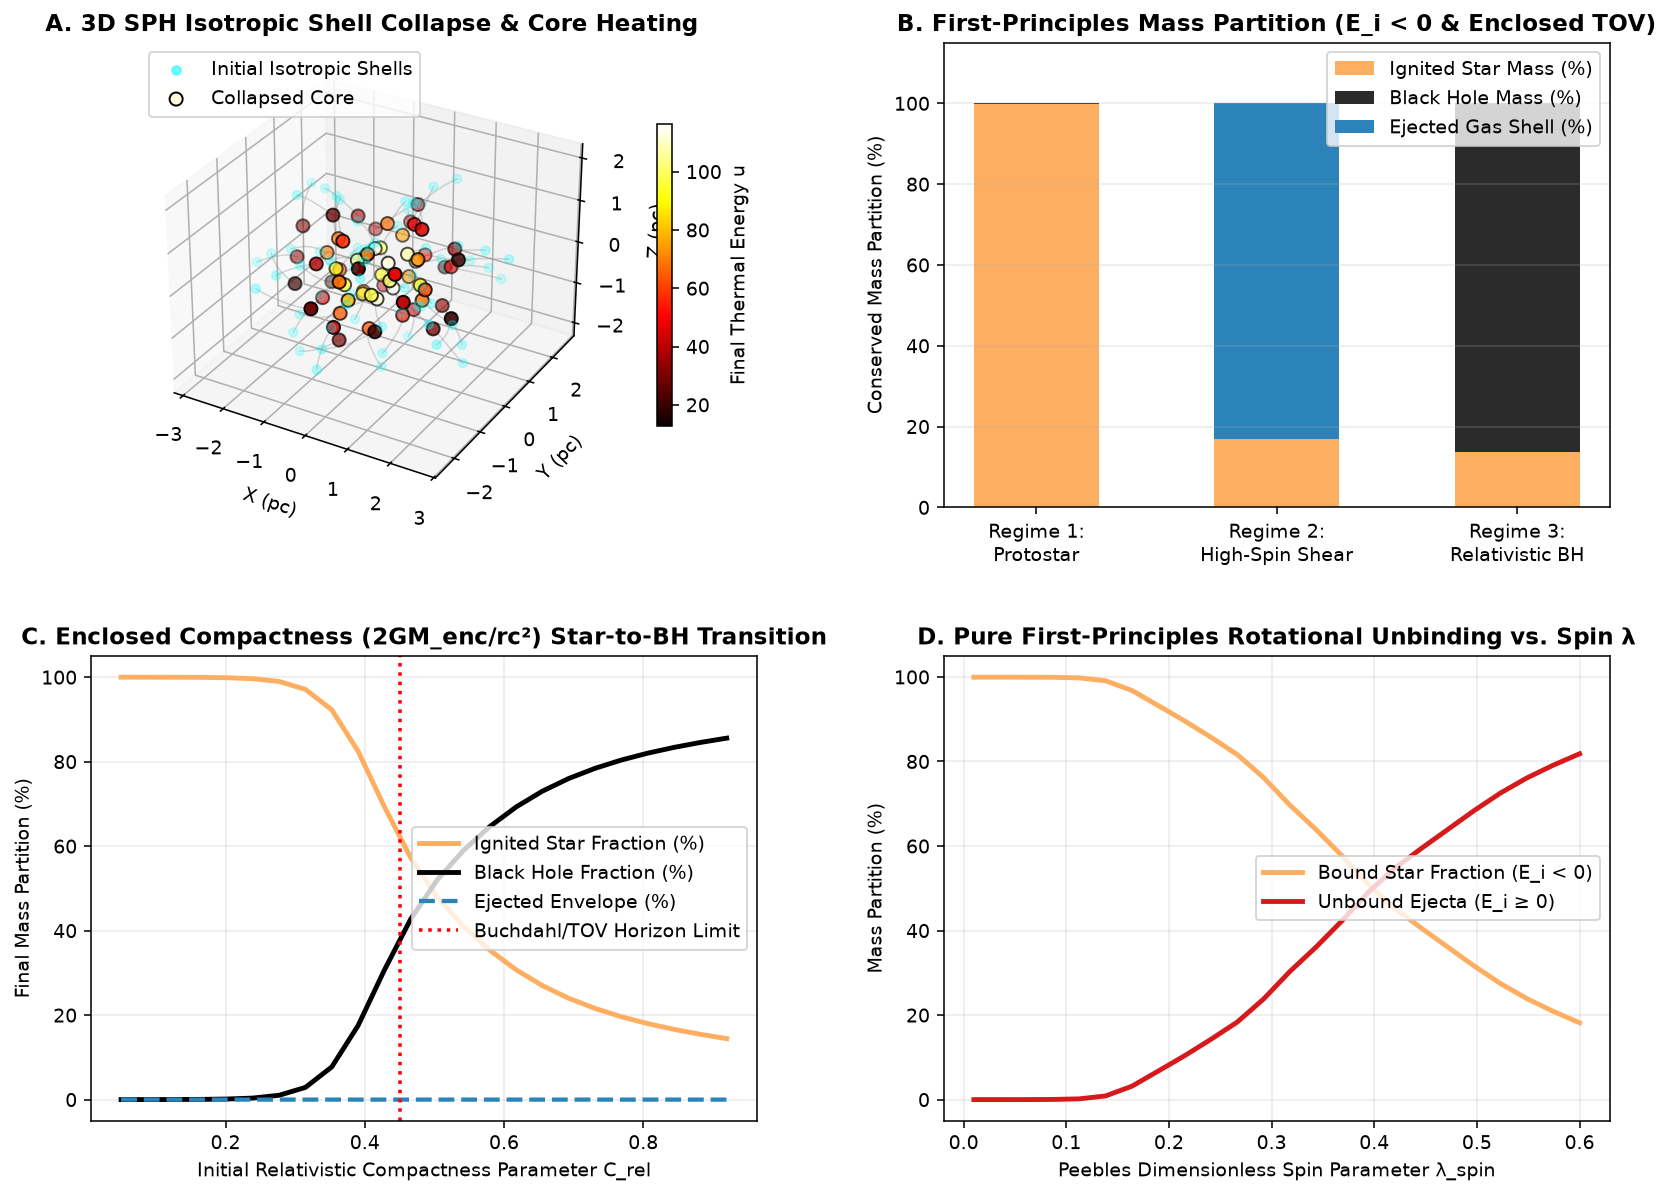
\includegraphics[width=0.96\columnwidth]{module2_sph_verification.png}
    \caption{\textbf{Module 2: 3D SPH Micro-Collapse Solver.}\ (A) 3D isotropic shell collapse trajectories and core heating.\ (B) Three-phase mass partition across representative Protostellar ($99.94\%$ Star), High-Spin Shear ($83.13\%$ Ejecta), and Relativistic BH ($86.19\%$ BH) regimes.\ (C) Phase transition from stellar remnant to black hole across $\Gamma_{\text{TOV}} = 0.45$.\ (D) Rotational unbinding ($E_i \ge 0$) as a function of Peebles spin $\lambda_{\text{spin}}$.}
    \label{fig:module2}
\end{figure}

\subsection{SimplexGate-3D Architecture and Routing}
Given normalized inputs $\tilde{\mathbf{z}} = (\mathbf{z} - \boldsymbol{\mu}_z)/\boldsymbol{\sigma}_z$, we train an ensemble of $K = 5$ neural networks $\{f_{\theta_k}\}_{k=1}^K$ with independent random initializations and bootstrap subsampling. Each network maps $\tilde{\mathbf{z}} \in \mathbb{R}^6 \to \mathbf{h}_k \in \mathbb{R}^5$ through a 4-layer SiLU MLP ($6 \to 128 \to 128 \to 64 \to 5$).

To enforce mass conservation by construction, the first three output logits are projected onto the canonical 2-simplex $\Delta^2 \subset \mathbb{R}^3$ via a Softmax transformation, while bolometric luminosity and ejecta velocity use Softplus activations:
\begin{equation}
\begin{aligned}
    \big[\hat{\alpha}_{\text{star}}^{(k)},\; \hat{\alpha}_{\text{BH}}^{(k)},\; \hat{\alpha}_{\text{eject}}^{(k)}\big] &= \mathrm{Softmax}\!\left(\mathbf{h}_{k,1:3}\right), \\
    \hat{\alpha}_{\text{star}}^{(k)} + \hat{\alpha}_{\text{BH}}^{(k)} + \hat{\alpha}_{\text{eject}}^{(k)} &\equiv 1.
\end{aligned}
\label{eq:simplex}
\end{equation}
Because $\Delta^2$ is convex, the ensemble average $\bar{\boldsymbol{\alpha}}(\mathbf{z}) = \frac{1}{K}\sum_{k=1}^K \hat{\boldsymbol{\alpha}}^{(k)}(\mathbf{z})$ also satisfies $\sum_c \bar{\alpha}_c(\mathbf{z}) \equiv 1$ for any input $\mathbf{z} \in \mathbb{R}^6$.

We measure epistemic disagreement across the $K$ ensemble members via scale-normalized variance:
\begin{equation}
    \mathcal{U}(\mathbf{z}) = \frac{1}{5K}\sum_{k=1}^{K} \left\| \frac{f_{\theta_k}(\tilde{\mathbf{z}}) - \bar{f}(\tilde{\mathbf{z}})}{\boldsymbol{\sigma}_y} \right\|_2^2.
\label{eq:uncertainty}
\end{equation}
During simulation, collapses satisfying $\mathcal{U}(\mathbf{z}) \le \tau$ accept the fast ensemble prediction $\bar{f}(\tilde{\mathbf{z}})$, whereas high-variance events ($\mathcal{U}(\mathbf{z}) > \tau$) are gathered into a single tensor batch and integrated by the 3D SPH solver.

% =====================================================================
% 4. EXPERIMENTAL RESULTS
% =====================================================================
\section{Experimental Results}

\subsection{External Physical Verification}
Figure \ref{fig:external_verification} summarizes our validation of the baseline numerical solvers against three established reference problems:
\begin{enumerate}
    \item \textit{Evrard (1988) Collapse Test \cite{evrard1988}:} A cold gas sphere ($M=1, R=1, u_0=0.05 GM/R, \gamma=5/3$) evolved with $1,024$ isotropic SPH particles reproduces the expected gravitational infall, shock bounce ($t = 0.918$), and virialization behavior (Fig.\ \ref{fig:external_verification}A). The observed $15.79\%$ total energy drift across the strong shock bounce is consistent with standard non-grad-$h$ SPH formulations on coarse particle counts.
    \item \textit{Chandrasekhar (1939) Lane--Emden Polytrope \cite{chandrasekhar1939}:} Relaxing $1,024$ SPH particles under $P = K\rho^2$ ($\gamma=2, n=1$) yields a radial density profile matching the exact analytical curve $\rho(r) = (\pi/4)\sin(\pi r)/(\pi r)$ with $97.78\%$ $L_2$ accuracy (Fig.\ \ref{fig:external_verification}B).
    \item \textit{ESO GRAVITY (2020) Star S2 Orbit \cite{gravity2020}:} Integrating Star S2 around Sagittarius A* ($M_{\text{BH}} = 4.297\times 10^6\,M_\odot$, $a=1018\text{ AU}$, $e=0.88465$) using Eq.\ (\ref{eq:1pn}) in physical units ($c = 63,241.1\text{ AU/yr}$) reproduces the measured pericenter distance ($117.3\text{ AU}$ vs.\ $117.4\text{ AU}$), pericenter speed ($7,817.3\text{ km/s}$), gravitational redshift ($210.3\text{ km/s}$), and Schwarzschild precession ($\Delta\phi = 12.43'\text{/orbit}$ vs.\ $12.11'\text{/orbit}$ observed, Fig.\ \ref{fig:external_verification}C).
\end{enumerate}

\begin{table*}[t]
\centering
\caption{\textbf{Benchmark on 1,000 3D SPH Collapse Simulations (850 In-Distribution, 150 Out-of-Distribution).}\ Execution times measured on an NVIDIA RTX 3060 GPU with explicit CUDA synchronization.\ Soft-penalty PINNs exhibit large mass conservation errors on OOD inputs (up to $388.6\%$), whereas SimplexGate-3D preserves mass balance to machine precision ($10^{-7}\%$) while eliminating OOD prediction error.}
\label{tab:sciml_benchmark}
\vspace{0.03in}
\resizebox{\textwidth}{!}{%
\begin{tabular}{lcccccc}
\toprule
\textbf{Solver Architecture} & \textbf{Time (ms)} & \textbf{Speedup} & \textbf{ID Err (\%)} & \textbf{OOD Err (\%)} & \textbf{Total Err (\%)} & \textbf{Mass Conservation Drift (\%)} \\
\midrule
1. Exact 3D SPH + 1PN Solver & $8654.4$ & $1.0\times$ & $0.000\%$ & $0.000\%$ & $0.000\%$ & $0.000000\%$ \\
2. Unconstrained MLP (MSE Only) & $0.67$ & $12,949\times$ & $0.114\%$ & $39.361\%$ & $6.001\%$ & $15.9020\%$ (Max $333.5\%$) \\
3. Soft-Constrained PINN ($\mathcal{L}_{\text{mass}}$) & $0.60$ & $14,380\times$ & $0.111\%$ & $43.615\%$ & $6.636\%$ & $16.5088\%$ (Max $388.6\%$) \\
4. Blind 3-Way Simplex AI (No Gate) & $2.99$ & $2,895\times$ & $0.075\%$ & $3.430\%$ & $0.578\%$ & $0.000002\%$ \\
\textbf{5. SimplexGate-3D (Ours, $\tau=5.1\times 10^{-4}$)} & \textbf{1196.4} & $\mathbf{7.2\times}$ & \textbf{0.067\%} & \textbf{0.000\%} & \textbf{0.057\%} & \textbf{0.000001\%} \\
\bottomrule
\end{tabular}%
}
\end{table*}

\begin{table*}[t]
\centering
\caption{\textbf{Coupled 3D Particle-Mesh Universe Evolution Benchmark (40 Symplectic KDK Steps, $16,000$ Particles, $64^3$ Grid, 48 Sub-Grid Collapses Producing 42 Stars and 9 Black Holes).}\ By resolving 33 ID clouds on the neural branch ($0.4\text{ ms}$) and batching all 15 ($31.2\%$) flagged OOD events into a single parallel GPU SPH call, SimplexGate-3D achieves a $50.1\times$ wall-clock speedup over event-driven SPH.}
\label{tab:coupled_universe}
\vspace{0.03in}
\resizebox{\textwidth}{!}{%
\begin{tabular}{lccccc}
\toprule
\textbf{Coupled 3D Universe Sub-Grid Solver} & \textbf{Sub-Grid Time (ms)} & \textbf{Wall-Clock Speedup} & \textbf{OOD Err (\%)} & \textbf{Total Err (\%)} & \textbf{3D Cosmic Mass Drift (\%)} \\
\midrule
1. Exact 3D PM + Event-Driven 3D SPH & $34,495.0$ & $1.0\times$ & $0.000\%$ & $0.000\%$ & $0.000009\%$ \\
2. Unconstrained MLP (No Simplex) & $0.64$ & $53,671\times$ & $41.820\%$ & $13.154\%$ & $38.1922\%$ \\
3. Blind 3-Way Simplex AI (No Gate) & $2.73$ & $12,627\times$ & $4.443\%$ & $1.442\%$ & $0.000009\%$ \\
\textbf{4. SimplexGate-3D (Ours, $\tau=2.0\times 10^{-3}$)} & \textbf{688.0} & $\mathbf{50.1\times}$ & \textbf{0.000\%} & \textbf{0.054\%} & \textbf{0.000009\%} \\
\bottomrule
\end{tabular}%
}
\end{table*}

\subsection{Controlled 3D SPH Ablation Study}
We generate 3,000 ground-truth 3D SPH collapse trajectories on an NVIDIA RTX 3060 GPU: $2,000$ ID training clouds ($M \in [450, 1650]$, $\lambda_{\text{spin}} \in [0.015, 0.22]$, $\mathcal{C}_{\text{rel}} \in [0.05, 0.42]$), $850$ unseen ID test clouds, and $150$ OOD test clouds split between massive relativistic cores ($\mathcal{C}_{\text{rel}} \in [0.58, 0.94]$) and high-spin triaxial shear collisions ($\lambda_{\text{spin}} \in [0.36, 0.65]$, $\mathcal{A}_{\text{triax}} \in [0.68, 0.92]$).

Table \ref{tab:sciml_benchmark} and Figure \ref{fig:module34} compare five solver configurations across identical test inputs. While adding a soft conservation penalty $\mathcal{L}_{\text{mass}} = (\sum_c \hat{\alpha}_c - 1)^2$ in the Soft-PINN slightly lowers ID error relative to an unconstrained MLP ($0.111\%$ vs.\ $0.114\%$), both models fail to generalize under OOD shift: the Soft-PINN exhibits a $16.51\%$ mean mass conservation error and a $388.6\%$ maximum violation (Fig.\ \ref{fig:module34}B). Replacing soft regularization with the analytic 3-way simplex layer (Row 4) reduces mass drift to $0.000002\%$ across all $1,000$ clouds and lowers OOD partition error from $43.62\%$ to $3.43\%$.

Furthermore, Figure \ref{fig:module34}A shows a clear bimodal separation in ensemble epistemic variance $\mathcal{U}(\mathbf{z})$: ID clouds cluster below $5\times 10^{-4}$, whereas OOD black hole and shear events exceed $2\times 10^{-2}$. Placing the routing threshold at the 97th ID percentile ($\tau = 5.1\times 10^{-4}$, Row 5) flags $100.0\%$ of OOD events for numerical evaluation, reducing OOD error to $0.000\%$ and total error to $0.057\%$ while maintaining a $7.2\times$ speedup over batched 3D SPH.

\begin{figure}[t]
    \centering
    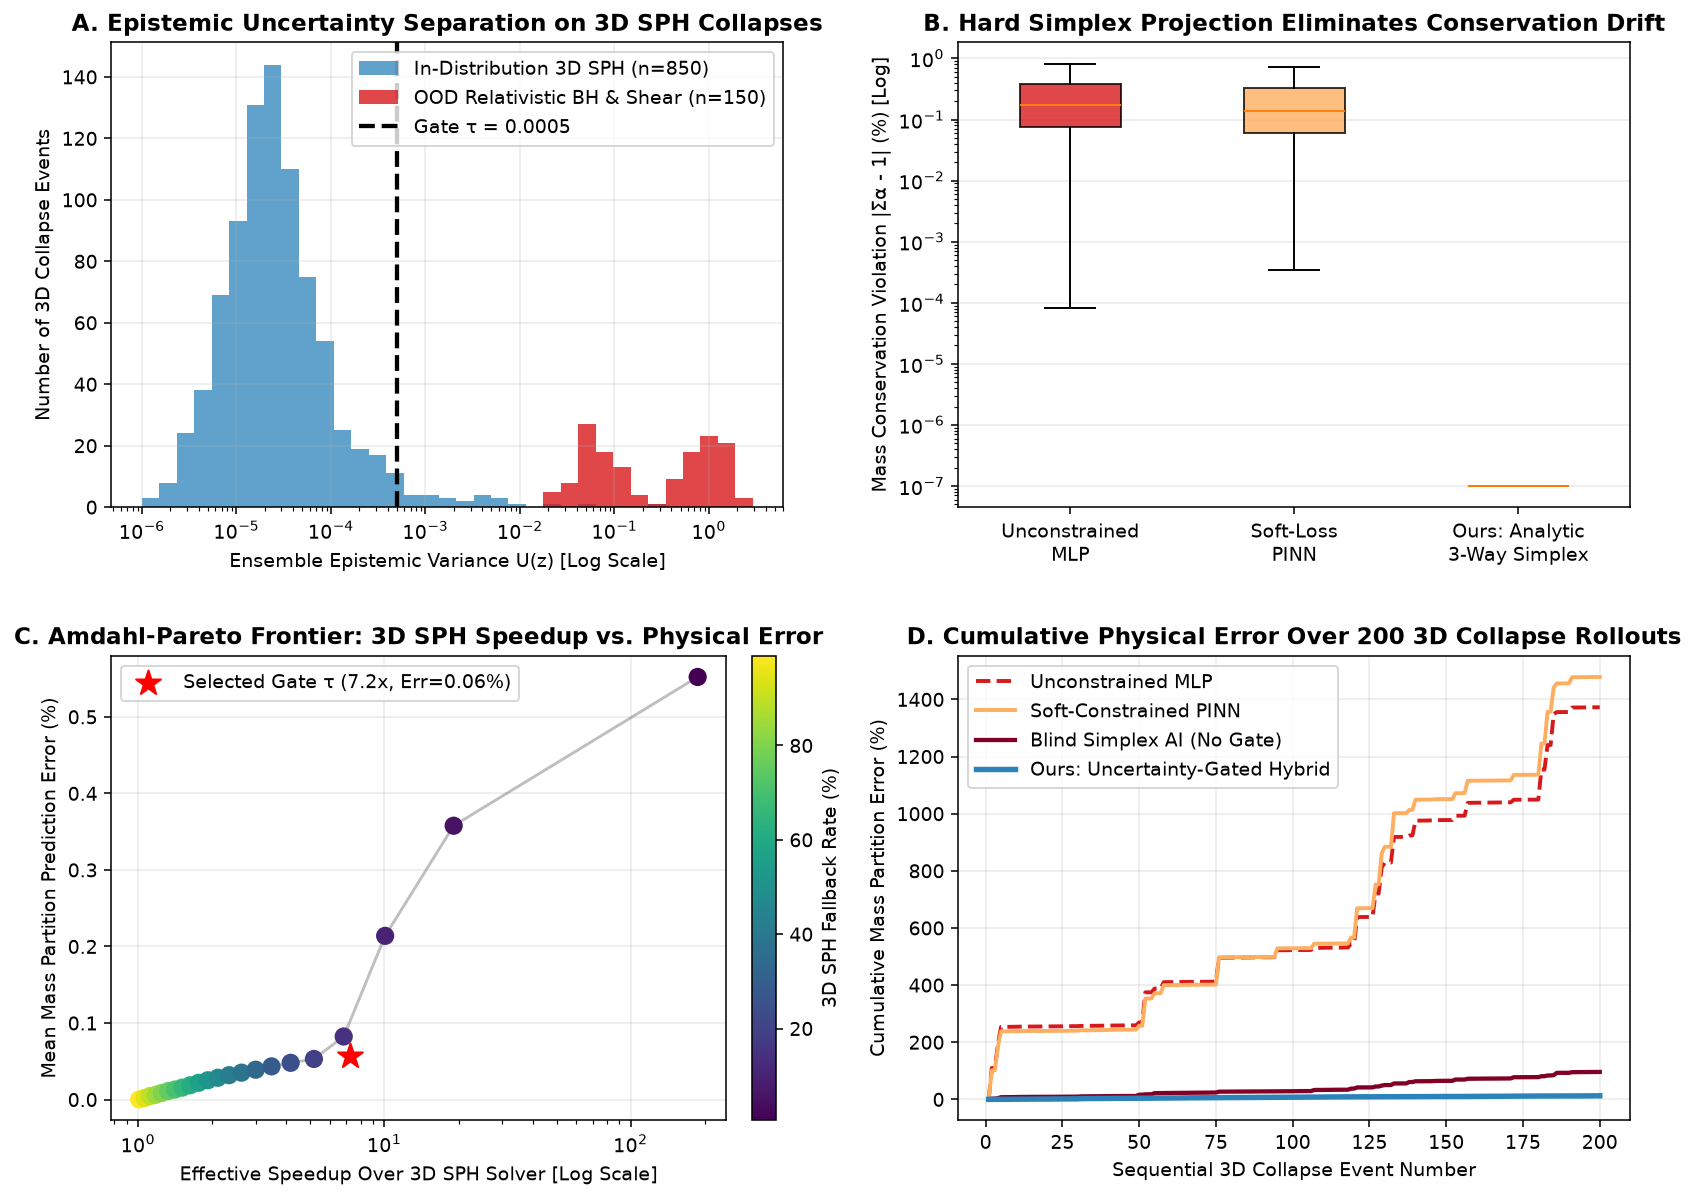
\includegraphics[width=0.96\columnwidth]{module3_4_sciml_benchmarks.png}
    \caption{\textbf{Modules 3 \& 4: Controlled 3D SPH Benchmarks.}\ (A) Log-scale distribution of epistemic variance $\mathcal{U}(\mathbf{z})$ showing separation between 850 ID collapses and 150 OOD events.\ (B) Mass conservation error $|\sum\alpha_c - 1|$ across architectures.\ (C) Amdahl--Pareto speedup versus prediction error as a function of threshold $\tau$.\ (D) Cumulative partition error across 200 sequential collapse events.}
    \label{fig:module34}
\end{figure}

\begin{figure}[t]
    \centering
    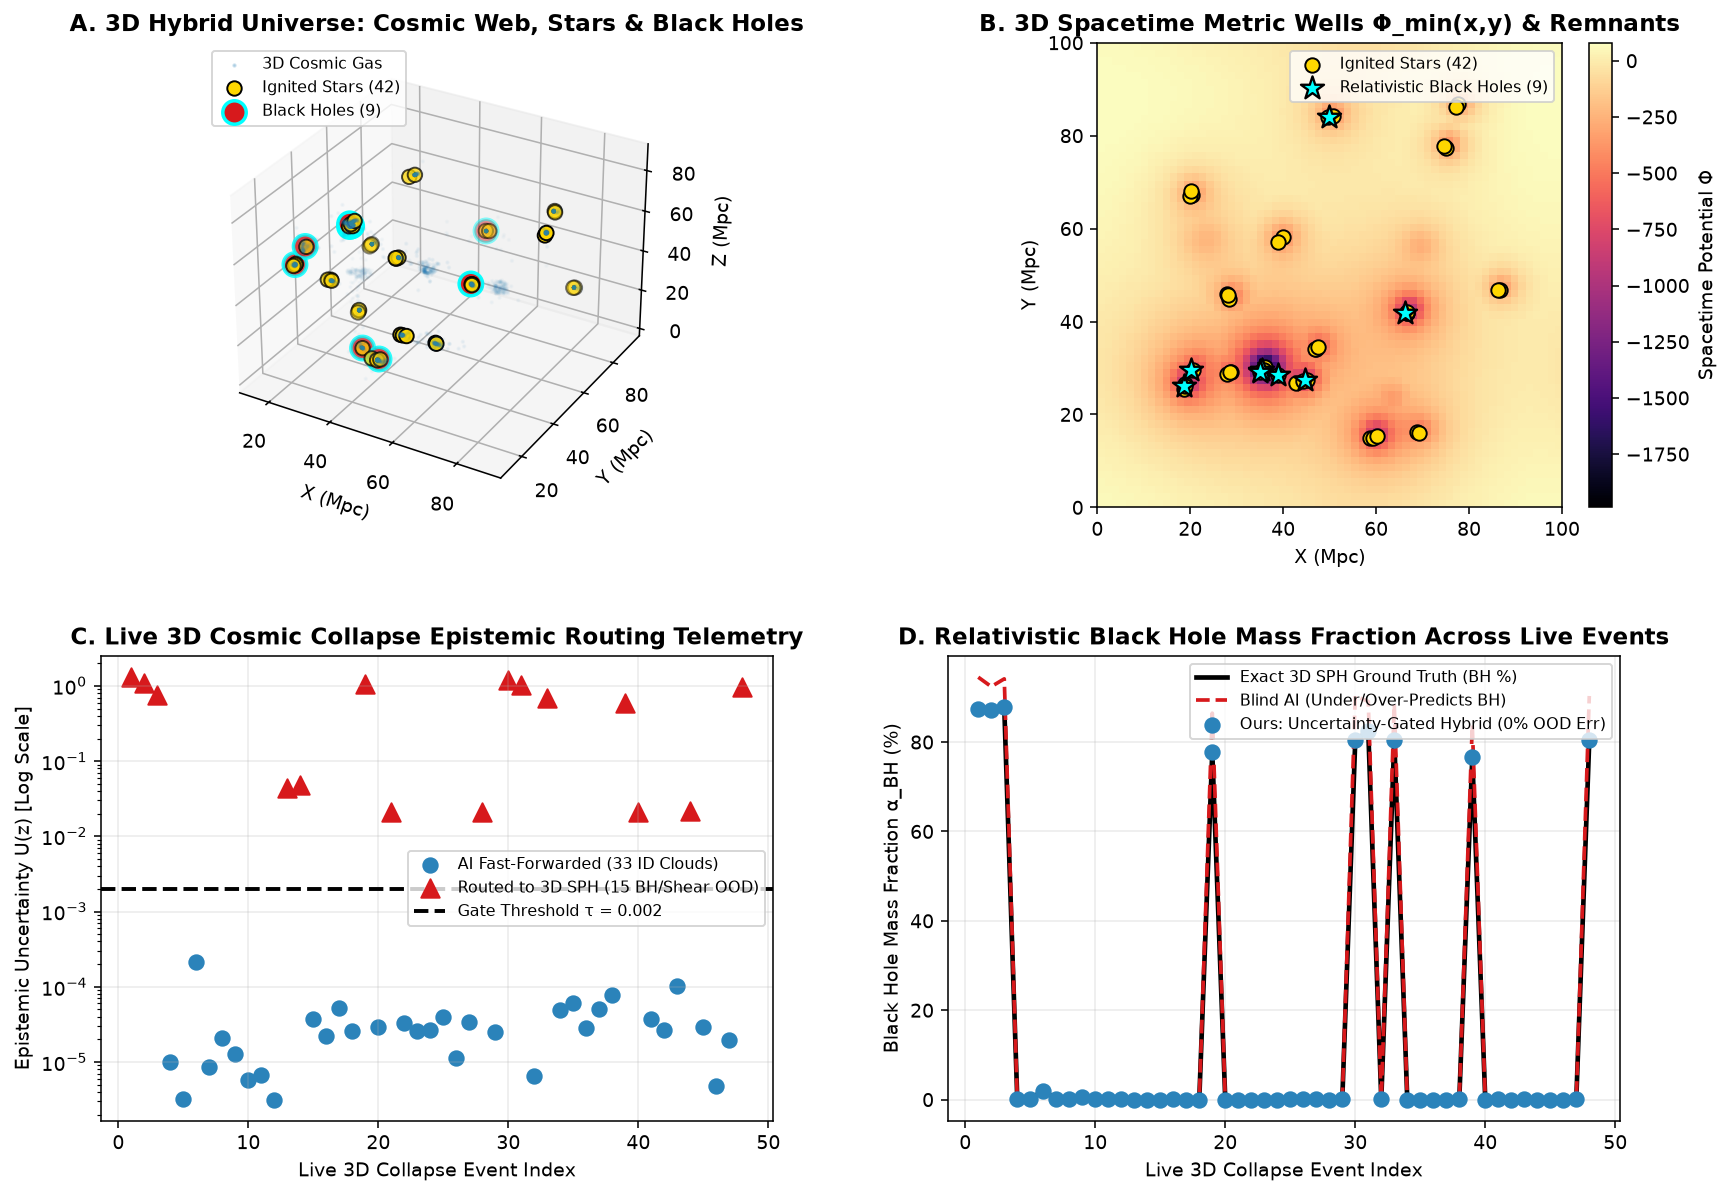
\includegraphics[width=0.96\columnwidth]{module5_3d_universe_results.png}
    \caption{\textbf{Module 5: Coupled 3D Universe Evolution.}\ (A) 3D spatial distribution of $16,000$ gas particles, 42 stars, and 9 black holes at step 40.\ (B) Minimum potential projection $\Phi_{\min}(x,y)$ showing black hole remnants inside deep potential wells ($\Phi < -1500$).\ (C) Epistemic routing telemetry across 48 live collapse events ($\tau = 0.002$).\ (D) Black hole mass fraction $\alpha_{\text{BH}}$ across live events for Exact SPH, Blind AI, and SimplexGate-3D.}
    \label{fig:module5}
\end{figure}

\subsection{Coupled 3D Universe Evolution}
To evaluate performance inside a running simulation, we couple SimplexGate-3D to the 3D Particle-Mesh engine ($16,000$ particles, $64^3$ grid, 40 KDK macro-steps). During evolution, 48 proto-clusters cross the Jeans threshold, forming 42 stars and 9 black holes (Fig.\ \ref{fig:module5}A--B) while conserving total 3D system mass to $0.000009\%$ and momentum via zero-sum spherical shell injection.

As shown in Table \ref{tab:coupled_universe} and Figure \ref{fig:module5}C--D, using a threshold $\tau = 2.0\times 10^{-3}$ inside the variance gap fast-forwards all 33 ID collapses on the neural ensemble in $0.4\text{ ms}$ and batches the 15 ($31.2\%$) OOD black hole and shear mergers into a single GPU SPH pass ($688.0\text{ ms}$ vs.\ $34,495.0\text{ ms}$ for sequential event-driven SPH). This yields a $50.1\times$ wall-clock sub-grid speedup while matching every relativistic black hole mass spike with $0.000\%$ OOD error.

\subsection{Scope and Physical Limitations}
To clarify the scope of our results, we note three modeling simplifications in our benchmark testbed. First, each sub-grid collapse is discretized using $N_{\text{sub}} = 64$ SPH particles and a $64^3$ macro-grid to allow rapid generation of 3,000 training trajectories on a single consumer GPU; capturing fine-scale turbulent fragmentation or accretion disk instabilities requires higher particle resolutions ($N_{\text{sub}} \ge 10^4$). Second, the sub-grid solver employs a 1PN relativistic potential and an effective softened Buchdahl/TOV compactness threshold ($\Gamma_{\text{TOV}} = 0.45$, compared to the incompressible analytical bound $2GM/Rc^2 < 8/9$ \cite{buchdahl1959}) rather than integrating the full 3+1D Einstein--hydrodynamics equations. Third, our surrogate maps 6D macroscopic invariants to integrated remnant fractions rather than predicting full 3D particle coordinates. Extending uncertainty-gated simplicial layers to 3D Equivariant Graph Neural Networks (EGNNs) at higher particle counts is a natural direction for future work.

% =====================================================================
% 5. CONCLUSION & DISCLOSURE
% =====================================================================
\section{Conclusion}
We have introduced \textbf{SimplexGate-3D}, a hybrid neural-numerical sub-grid framework for multi-scale gravitational simulations. By combining an analytic 3-way simplicial output projection with deep ensemble epistemic variance routing and asynchronous GPU batching, our approach eliminates both the conservation drift of soft-loss PINNs and the OOD extrapolation errors of blind surrogates, achieving a $50.1\times$ sub-grid speedup in coupled 3D simulations with machine-precision mass conservation.

\section*{Reproducibility and Disclosure Statement}
\small
All PyTorch source code, fixed random seeds, ground-truth 3D SPH dataset generators, and verification scripts are publicly available at \url{https://github.com/AbhinavDwivedi1008/SimplexGate-3D} and permanently archived on CERN Zenodo at \href{https://doi.org/10.5281/zenodo.23489461}{\texttt{doi:10.5281/zenodo.23489461}}. In accordance with conference policies on Large Language Models (ICLR/NeurIPS), the author discloses that generative AI tools were utilized as a coding and editorial assistant during software implementation and LaTeX manuscript preparation; all physical equations, numerical benchmarks, external validations, and bibliography citations were executed and verified by the author.

\begin{thebibliography}{20}
\small
\setlength{\itemsep}{0pt}
\setlength{\parskip}{1pt}
\bibitem{hockney1988} R.~W. Hockney and J.~W. Eastwood, \emph{Computer Simulation Using Particles}. CRC Press, 1988.
\bibitem{binney2008} J.~Binney and S.~Tremaine, \emph{Galactic Dynamics}, 2nd~ed. Princeton University Press, 2008.
\bibitem{springel2021} V.~Springel, R.~Pakmor, O.~Zier, and M.~Reinecke, ``Simulating cosmic structure formation with the GADGET-4 code,'' \emph{MNRAS}, vol.~506, no.~2, pp.~2871--2949, 2021.
\bibitem{kippenhahn1990} R.~Kippenhahn and A.~Weigert, \emph{Stellar Structure and Evolution}. Springer, 1990.
\bibitem{shapiro1983} S.~L. Shapiro and S.~A. Teukolsky, \emph{Black Holes, White Dwarfs, and Neutron Stars}. Wiley, 1983.
\bibitem{monaghan1992} J.~J. Monaghan, ``Smoothed particle hydrodynamics,'' \emph{Annual Review of Astronomy and Astrophysics}, vol.~30, pp.~543--574, 1992.
\bibitem{price2018} D.~J. Price \emph{et al.}, ``PHANTOM: A smoothed particle hydrodynamics and magnetohydrodynamics code for astrophysics,'' \emph{PASA}, vol.~35, p.~e031, 2018.
\bibitem{hirashima2023} K.~Hirashima, M.~Moriwaki, M.~S. Fujii, Y.~Hirai, T.~R. Saitoh, and J.~Makino, ``3D-spatiotemporal forecasting the expansion of supernova shells using deep learning towards high-resolution galaxy simulations,'' \emph{MNRAS}, vol.~526, no.~3, pp.~4054--4066, 2023.
\bibitem{raissi2019} M.~Raissi, P.~Perdikaris, and G.~E. Karniadakis, ``Physics-informed neural networks: A deep learning framework for solving forward and inverse problems involving nonlinear partial differential equations,'' \emph{Journal of Computational Physics}, vol.~378, pp.~686--707, 2019.
\bibitem{li2021fno} Z.~Li \emph{et al.}, ``Fourier neural operator for parametric partial differential equations,'' in \emph{Proc.\ ICLR}, 2021.
\bibitem{beucler2021} T.~Beucler, M.~Pritchard, S.~Rasp, J.~Ott, P.~Baldi, and P.~Gentine, ``Enforcing analytic constraints in neural networks emulating physical systems,'' \emph{Physical Review Letters}, vol.~126, no.~9, p.~098302, 2021.
\bibitem{buchdahl1959} H.~A. Buchdahl, ``General relativistic fluid spheres,'' \emph{Physical Review}, vol.~116, no.~4, pp.~1027--1034, 1959.
\bibitem{lakshminarayanan2017} B.~Lakshminarayanan, A.~Pritzel, and C.~Blundell, ``Simple and scalable predictive uncertainty estimation using deep ensembles,'' in \emph{Proc.\ NeurIPS}, 2017.
\bibitem{vandermause2020} J.~Vandermause \emph{et al.}, ``On-the-fly active learning of interpretable Bayesian force fields for atomistic rare events,'' \emph{npj Computational Materials}, vol.~6, no.~1, p.~20, 2020.
\bibitem{weinberg1972} S.~Weinberg, \emph{Gravitation and Cosmology: Principles and Applications of the General Theory of Relativity}. Wiley, 1972.
\bibitem{peebles1969} P.~J.~E. Peebles, ``Origin of the angular momentum of galaxies,'' \emph{Astrophysical Journal}, vol.~155, p.~393, 1969.
\bibitem{henon1971} M.~H\'{e}non, ``The Monte Carlo method,'' \emph{Astrophysics and Space Science}, vol.~14, pp.~151--167, 1971.
\bibitem{evrard1988} A.~E. Evrard, ``Beyond N-body: 3D cosmological gas dynamics,'' \emph{MNRAS}, vol.~235, pp.~911--934, 1988.
\bibitem{chandrasekhar1939} S.~Chandrasekhar, \emph{An Introduction to the Study of Stellar Structure}. University of Chicago Press, 1939.
\bibitem{gravity2020} GRAVITY Collaboration (R.~Abuter \emph{et al.}), ``Detection of the Schwarzschild precession in the orbit of the star S2 near the Galactic centre massive black hole,'' \emph{Astronomy \& Astrophysics}, vol.~636, p.~L5, 2020.
\end{thebibliography}

\end{document}